\part{IoT platform}
\chapter{Node-RED}
\section{Node-RED: En Teknisk Gennemgang}
\subsection{Introduktion til Node-RED}
Node-RED er et kraftfuldt udviklingsværktøj baseret på flow-baseret programmering, primært anvendt til at forbinde hardwareenheder, API'er og online-tjenester på nye og innovative måder. Det blev udviklet af IBM og er bygget på Node.js, hvilket gør det platform-uafhængigt, skalerbart og velegnet til IoT (Internet of Things) applikationer. Node-RED leverer en webbaseret editor, der gør det muligt for brugere at oprette JavaScript-funktioner og forbinde noder for at skabe flows. Disse flows kan interagere med forskellige protokoller og hardware, hvilket gør Node-RED til et alsidigt værktøj til IoT og automatiseringsopgaver. 

\begin{figure}[h!]
	\centering
	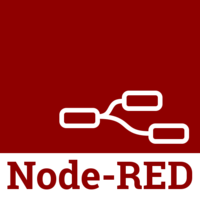
\includegraphics[width=0.7\textwidth]{fig/fig26.png} % A high-level architecture diagram of Node-RED
	\caption{Node-RED}
\end{figure}

\subsection{Arkitektur og Kernekomponenter}
Node-RED's arkitektur er modulær og består af tre primære komponenter:

\subsubsection{Node-RED Runtime}
Runtime-miljøet er bygget på Node.js og er ansvarligt for at eksekvere flows, håndtere noder og håndtere meddelelser mellem noder. Det opererer inden for en enkelt-trådet event loop, typisk for Node.js-applikationer, hvilket muliggør asynkron behandling og non-blocking operationer. Runtime-miljøet indlæser flow-definitioner fra en JSON-fil og administrerer eksekveringen af noder, når meddelelser passerer gennem flowet. Det giver også API'er til at oprette, slette og administrere flows programmatisk.

\subsubsection{Node-RED Editor}
Node-RED editoren er en webbaseret grænseflade, der bruges til at udvikle flows. Den tilbyder en drag-and-drop grænseflade, hvor brugere kan placere noder på en arbejdsflade og forbinde dem for at definere dataflowet.

\begin{figure}[h!]
	\centering
	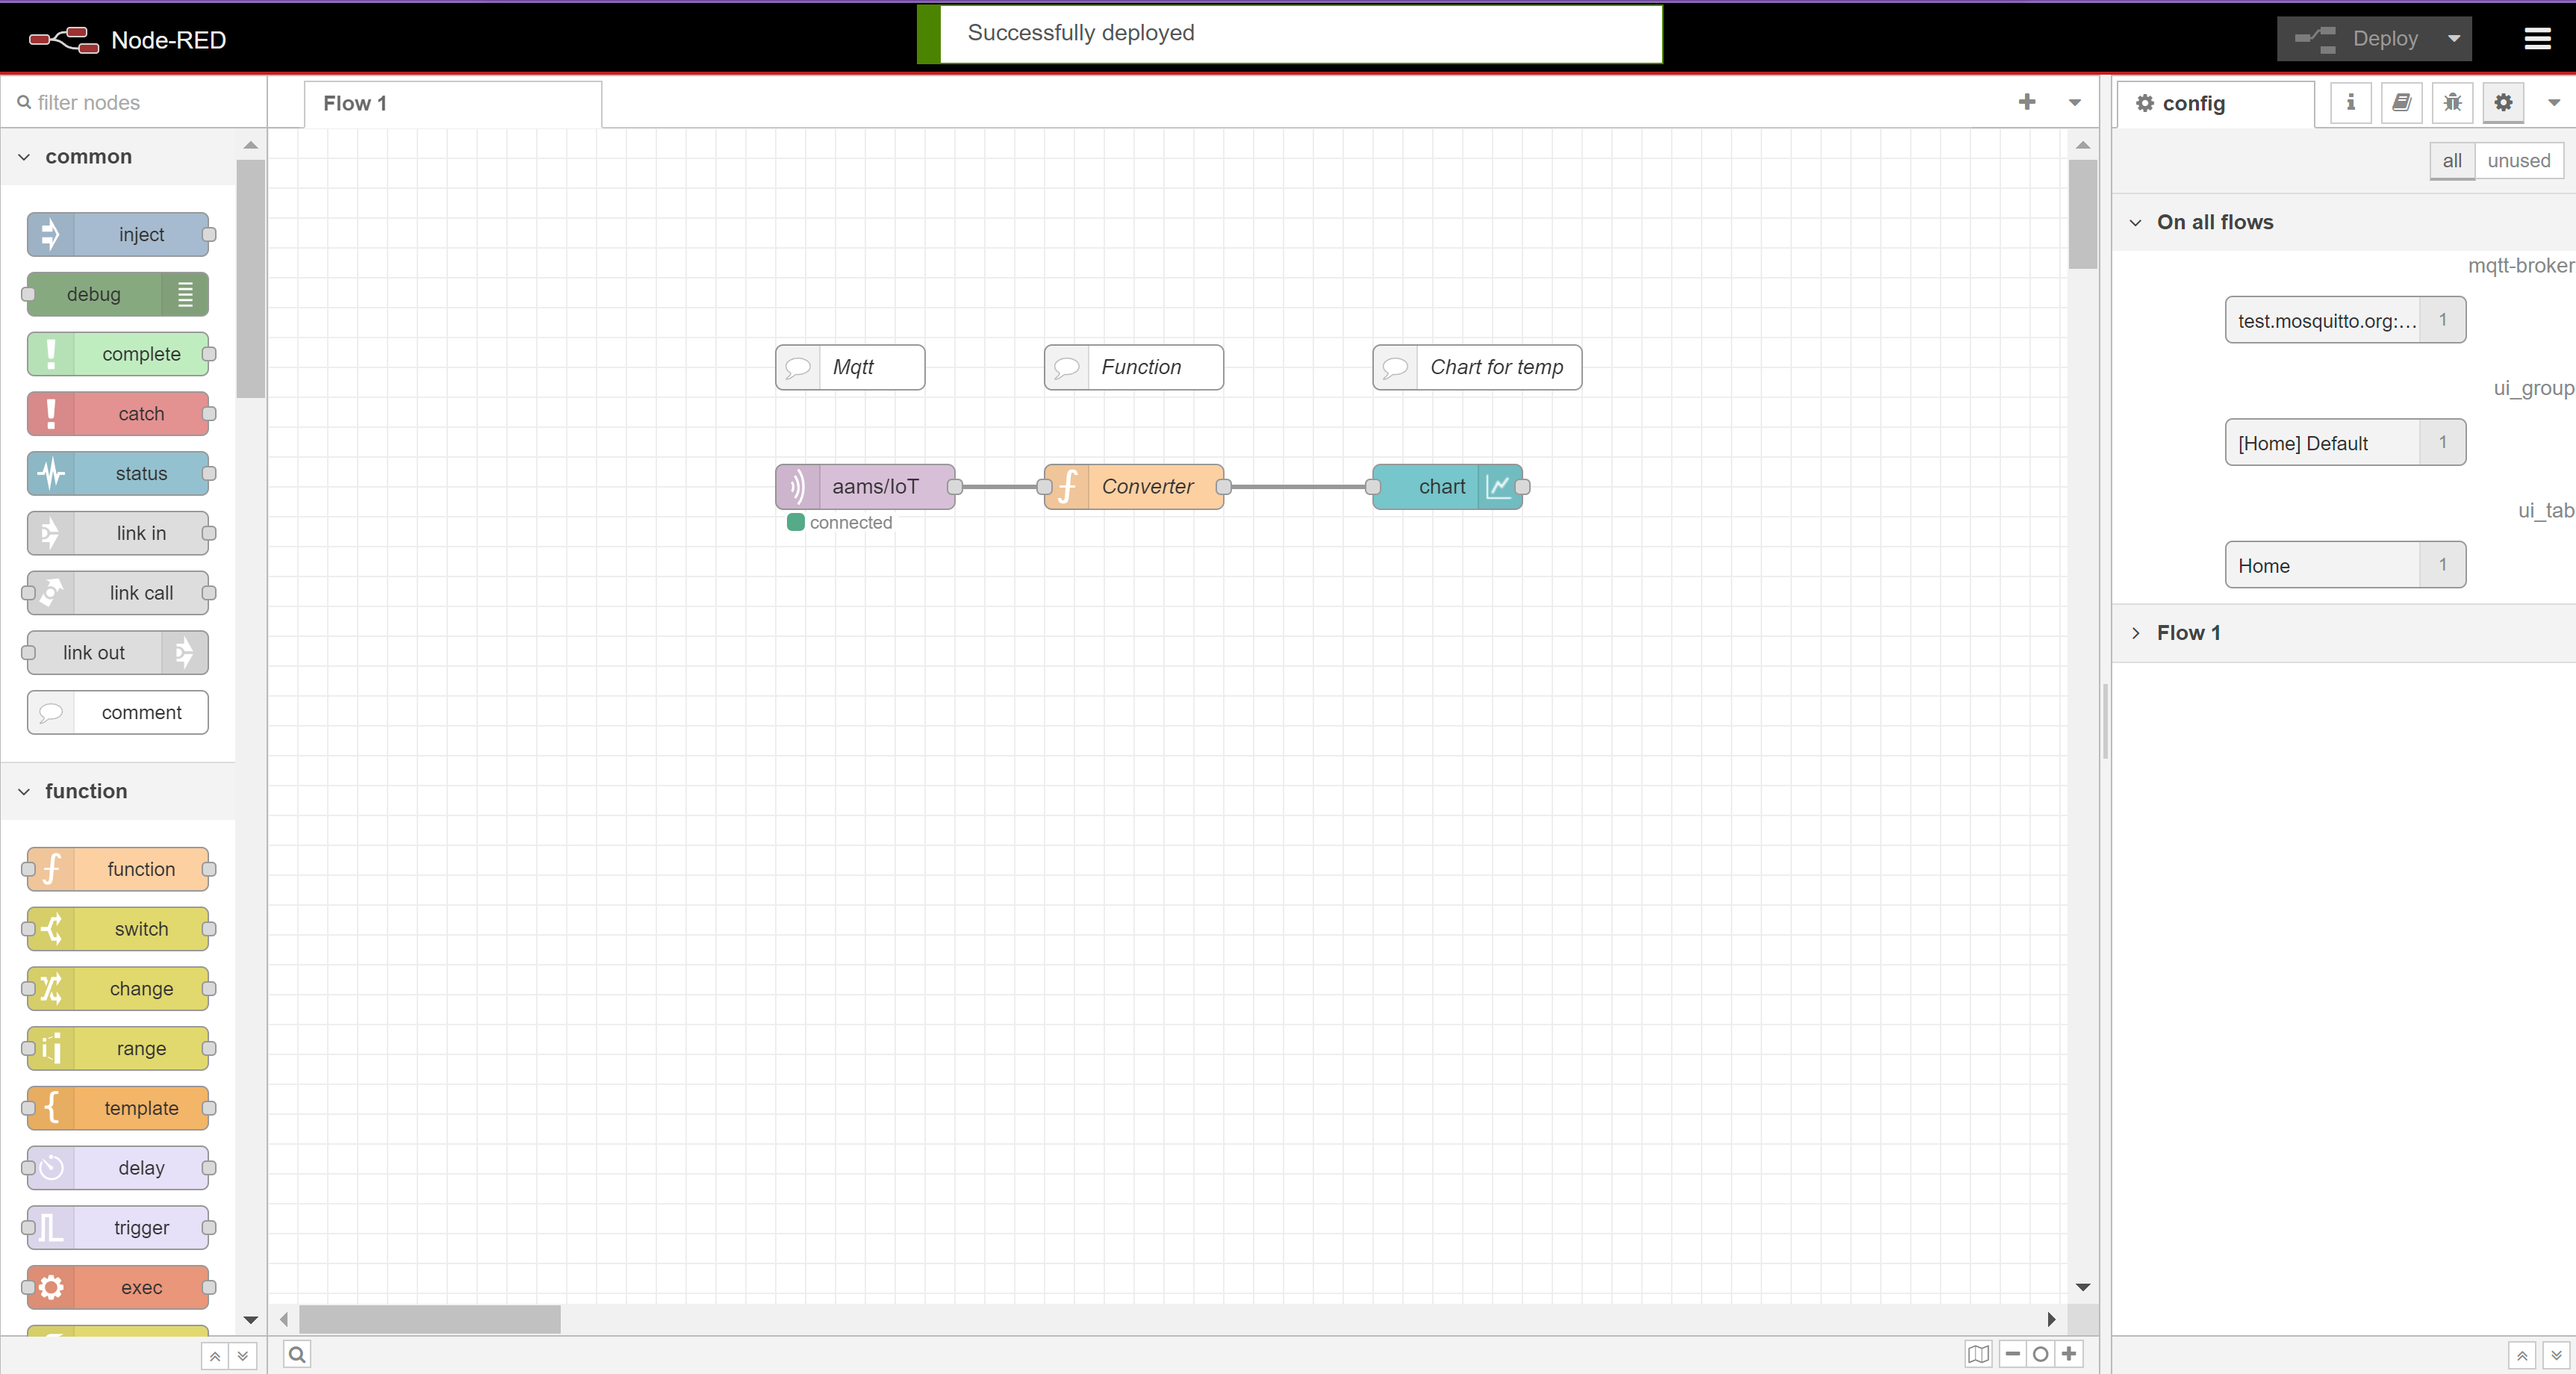
\includegraphics[width=\textwidth]{fig/fig25.png} % A screenshot of the Node-RED web-based editor with a simple flow
	\caption{Node-RED editoren med et simpelt flow, hvor noder er trukket ind i arbejdsområdet og forbundet.}
\end{figure}
\noindent Editorens kommunikation med runtime-miljøet sker via WebSocket og HTTP-protokoller, hvilket muliggør realtidsopdateringer og interaktion med kørende flows. Editorens output er JSON-baserede flow-definitioner, som derefter eksekveres af runtime-miljøet.

\subsubsection{Noder}
Noder er de grundlæggende byggeklodser i Node-RED. Hver node repræsenterer en specifik funktion, input, output eller serviceintegration. Noder kategoriseres i kerne-noder (som er indbygget i Node-RED) og bidrags-noder (som er tilgængelige via Node-RED-biblioteket). Noder kommunikerer ved at sende meddelelser til hinanden. Disse meddelelser er JavaScript-objekter, der kan indeholde data, konfigurationsindstillinger og metadata. Noder kan ændre, dirigere eller oprette meddelelser, mens de eksekverer.

\subsection{Flow-baseret Programmeringsparadigme}
Node-RED anvender et flow-baseret programmeringsparadigme, hvor udviklere opbygger applikationer ved at skabe flows eller grafer af noder, der repræsenterer behandlingsskridt. Hver node i et flow udfører en specifik opgave, såsom at læse sensordata, behandle dem og sende resultaterne til en database eller en ekstern API.

\subsubsection{Meddelelsesflow}
I Node-RED flyder meddelelser mellem noder langs definerede stier. Hver node behandler indkommende meddelelser og bestemmer, hvordan de skal ændres eller dirigeres til efterfølgende noder.

\subsubsection{Funktionsnoder}
For brugerdefineret logik tilbyder Node-RED funktionsnoder, hvor udviklere kan skrive JavaScript-kode. Dette muliggør kompleks databehandling, transformation og kontrollogik inden for et flow.

\subsection{Implementering og Skalerbarhed}
Node-RED er designet til at køre på en bred vifte af platforme, fra små enheder som Raspberry Pi til cloud-baserede tjenester. Implementering kan være så simpelt som at køre en lokal instans på en enkelt maskine eller at implementere i et cloud-miljø ved hjælp af Docker eller andre containerteknologier.

\subsubsection{Skalerbarhed}
Node-RED's event-drevne, non-blocking arkitektur gør det iboende skalerbart. Det kan håndtere flere forbindelser og høj-throughput datastreams, hvilket gør det velegnet til store IoT-implementeringer.

\subsubsection{Clustering}
Selvom Node-RED ikke selv understøtter clustering, kan det implementeres i et klynge-miljø ved hjælp af værktøjer som Kubernetes, hvilket muliggør skalering på tværs af flere noder og fejltolerance.

\subsection{Integration med IoT Protokoller og Tjenester}
Node-RED er særligt kraftfuldt inden for IoT på grund af dets omfattende understøttelse af forskellige protokoller og tjenester:

\subsubsection{MQTT}
Node-RED understøtter naturligt MQTT (Message Queuing Telemetry Transport), en letvægtsbeskedsprotokol, der ofte anvendes i IoT. MQTT-noder kan bruges til at abonnere på emner, publicere meddelelser og integrere med MQTT-brokers.

\subsubsection{HTTP og WebSocket}
Node-RED tilbyder noder til håndtering af HTTP og WebSocket-kommunikation, hvilket muliggør integration med webtjenester, RESTful API'er og realtidsapplikationer.

\subsubsection{Modbus, OPC-UA og Andre Industrielle Protokoller}
Til industrielle IoT-applikationer (IIoT) tilbyder Node-RED noder til interaktion med Modbus, OPC-UA og andre industrielle protokoller. Dette muliggør interface med PLC'er, SCADA-systemer og andet industrielt udstyr.

\subsubsection{Cloud Tjenester}
Node-RED kan integrere med cloud-tjenester såsom AWS, Azure og Google Cloud, hvilket tillader data at blive sendt til cloud-databaser, behandlet af cloud-funktioner eller visualiseret ved hjælp af cloud-dashboards.

\subsection{Sikkerhed og Godkendelse}
Sikkerhed er et kritisk aspekt af enhver IoT-implementering, og Node-RED tilbyder flere mekanismer til at sikre sikker drift:

\subsubsection{Brugergodkendelse}
Node-RED kan konfigureres til at kræve brugergodkendelse for adgang til editoren og API'er. Dette gøres typisk ved hjælp af HTTP basic authentication eller ved integration med eksterne godkendelsesudbydere.

\subsubsection{TLS/SSL}
Node-RED understøtter TLS/SSL-kryptering for at sikre HTTP, WebSocket og MQTT-kommunikation. Dette sikrer, at data, der sendes til og fra Node-RED, er beskyttet mod aflytning og manipulation.

\subsection{Udvidelsesmuligheder og Custom Noder}
Node-RED er designet til at være fleksibelt og udvidelsesbart. Ud over de mange indbyggede noder kan udviklere oprette og dele deres egne custom noder.

\subsubsection{Oprettelse af Custom Noder}
Udviklere kan oprette custom noder ved hjælp af JavaScript og Node.js-økosystemet. Disse noder kan derefter integreres i Node-RED editoren og bruges sammen med eksisterende noder.

\chapter{Opgaver}
\section{Modtagelse af Seriel Data fra ESP32 i Node-RED}
I denne sektion beskrives processen for, hvordan man kan opsætte og modtage seriel data fra en ESP32-mikrocontroller til Node-RED. Seriel kommunikation er en simpel og effektiv måde at overføre data mellem enheder, og ved at integrere dette med Node-RED, kan dataene nemt visualiseres, behandles eller videresendes.

\subsection{Opsætning af Seriel Kommunikation}
For at opsætte seriel kommunikation mellem ESP32 og Node-RED skal følgende trin følges:

\begin{enumerate}
	\item \textbf{Forbind ESP32 til Computeren:} Start med at forbinde din ESP32 til din computer via USB. Dette vil oprette en seriel forbindelse, som både ESP32 og Node-RED kan kommunikere over.
	
	\item \textbf{Installér Serial Node i Node-RED:} Åbn Node-RED og installér \texttt{node-red-node-serialport}, hvis det ikke allerede er installeret. Dette bibliotek giver adgang til at læse og skrive seriel data i Node-RED.
	
	\item \textbf{Tilføj og Konfigurer en Serial In Node:} Træk en \texttt{serial in} node ind i dit flow i Node-RED. Konfigurer noden til at lytte på den serielle port, som din ESP32 er tilsluttet. Sørg for, at baudraten og andre kommunikationsparametre matcher dem, der er indstillet på ESP32.
	
	\item \textbf{Tilføj en Debug Node:} For at kunne se de data, som modtages via den serielle port, tilføj en \texttt{debug} node og forbind den til \texttt{serial in} noden. Dette vil vise de modtagne data i Node-RED's debug-vindue.
	
	\item \textbf{Programmering af ESP32:} Upload en simpel skitse til din ESP32, der sender data via seriel kommunikation. Dette kan være så simpelt som at sende en tekststreng eller sensordata hver gang en bestemt hændelse indtræffer.
	
	\item \textbf{Kør Flowet i Node-RED:} Når alle trin er fulgt, kan du køre dit flow i Node-RED. Data, der sendes fra ESP32, vil nu kunne ses i debug-vinduet i Node-RED.
	
\end{enumerate}
Denne proces sikrer, at data fra din ESP32 kan modtages og håndteres i Node-RED, hvilket gør det muligt at integrere enheder og sensorer i dit IoT-netværk.

\subsection{Opgave: Modtagelse og Visualisering af Temperaturdata fra ESP32 i Node-RED}
\noindent \textbf{Mål:} Konfigurer Node-RED til at modtage seriel data fra en ESP32, som sender temperaturmålinger, og visualiser dataene i Node-RED's dashboard.

\subsubsection*{Opgavebeskrivelse:}
\begin{enumerate}
	\item \textbf{Forberedelse:}
	\begin{itemize}
		\item Installer \texttt{node-red-node-serialport} i Node-RED.
		\item Sørg for, at din ESP32 er forbundet til din computer via USB.
		\item Upload en skitse til ESP32, der måler temperaturen (f.eks. med en DHT11-sensor) og sender dataene via den serielle port.
	\end{itemize}
	
	\item \textbf{Implementering:}
	\begin{itemize}
		\item Tilføj en \texttt{serial in} node i Node-RED og konfigurer den til at læse data fra den korrekte serielle port.
		\item Tilføj en \texttt{debug} node for at sikre, at dataene modtages korrekt.
		\item Tilføj en \texttt{chart} node i Node-RED's dashboard for at visualisere temperaturdataene.
		\item Forbind noderne i Node-RED, så dataene flyder fra \texttt{serial in} noden til \texttt{chart} noden via en funktion eller \texttt{change} node for at formatere dataene korrekt.
	\end{itemize}
	
	\item \textbf{Test:}
	\begin{itemize}
		\item Start flowet i Node-RED og verificer, at temperaturdataene modtages korrekt og vises i dashboardet.
		\item Juster om nødvendigt dataformatet eller baudraten for at sikre, at al kommunikation sker uden fejl.
	\end{itemize}
\end{enumerate}
\noindent \textbf{Formål:} Formålet med denne opgave er at lære at opsætte seriel kommunikation mellem en ESP32 og Node-RED, samt hvordan man kan visualisere sensor data i et brugervenligt dashboard.